\documentclass[onecolumn,preprintnumbers,amsmath,amssymb,superscriptaddress]{revtex4}
%\usepackage[pdftex]{graphicx}

\usepackage{amsmath,amsfonts,amssymb}
\usepackage[english]{babel}
\usepackage[latin1]{inputenc}
\usepackage[T1]{fontenc}
\usepackage{color}
\usepackage{float}
\usepackage{verbatim}
\usepackage{graphicx}
\usepackage{bm}
\usepackage{mathtools}
\usepackage{stmaryrd}
\usepackage{anyfontsize}

%\usepackage{caption}
\usepackage{subcaption}
\usepackage{graphicx}

%\usepackage{epstopdf}
%\usepackage{array}
%\usepackage{tabularx}
%\usepackage{multirow}
\usepackage{color}
%\usepackage{multibox}
%\usepackage{rotating}
%\usepackage{lineno}
%\usepackage[left]{lineno}
%\usepackage[comma,sort&compress]{natbib}
%\usepackage{authblk}
%\usepackage{multicol}

%\bibliographystyle{ieeetr}


%\linenumbers
%\setlength\linenumbersep{3pt}

\begin{document}


%\title{Simple rules yield complex communities: deconstructed species interactions and the assembly of communities}
%\title{Community assembly and dynamics by the deconstruction of species interactions}
\title{Salmon straying description}
%\author{Justin D. Yeakel${}^{1,2,*}$, Christopher P. Kempes${}^{2}$, \& Sidney Redner${}^{2,3}$ \\ \\
%${}^1$School of Natural Science, University of California Merced, Merced, CA \\
%${}^2$The Santa Fe Institute, Santa Fe, NM \\
%${}^3$Department of Physics, Boston University, Boston MA \\
%${}^*$To whom correspondence should be addressed: jdyeakel@gmail.com
%}



\maketitle



\section*{Introduction}


\section*{Model Description}

Here we consider two populations $N_1$ and $N_2$ that are separated in space, each with trait values $x_1$ and $x_2$ determining recruitment rates.
We assume that there is an optimum trait value $\theta_1$ and $\theta_2$ associated with each habitat, where recruitment is maximized if the trait value of the local population $x = \theta$.
Moreover, we assume that $x_{1,2}$ are normally distributed with means $\mu_1$ and $\mu_2$ and have a shared standard deviation $\sigma$.
As such, the recruitment rate for both populations is determined by the mean trait value of the local population, such that $r_1 = R_1[\mu_1(t)|\theta_1]$.
Trait means for each population are subject to selection, the strength of which depends on the difference between the population mean and the local trait optimum at a given point in time.

The two populations are assumed to reproduce in spatially separate sites that are close enough such that a proportion of the population $m$ can stray into the wrong site, and where mortality occurs before individuals return to spawn.
If there is no straying between these populations (such that they are independent), then the mean trait evolves towards the optimal value such that $x_1 \rightarrow \theta_1$, and the recruitment rate for that population will be maximized.
If there is straying between populations at rate $m$, then the traits in each respective location will be pulled away from the optimum, and recruitment rates will be lowered.
As $m \rightarrow 0.5$, the populations are perfectly mixed, acting as a single population.


We use the discrete Ricker population dynamic framework described by Shelton and Mangel \cite{} as the basis for our two-site model, with the added effect of the local population $N_i$ mixing with a set proportion $m$ of a remote population $N_j$ that is straying into it.
We first assume that the proportion ${\rm e}^{-Z}$ of both populations survive, and that the aggregated mix of the populations (local individuals in addition to the straying individuals) are subject to the same compensatory effects, determined by the parameter $\beta$.
For a local site $i\in(1,2)$ that collects straying individuals from a remote site $j\in(1,2)$, if $N_i$ is the local site and $N_j$ is the remote site, the difference equation that determine changes in population size is

\begin{align}
  N_i(t+1) &= \left((1-m)N_i(t) + m N_j(t) \right){\rm e}^{-Z} \\ \nonumber
  &+ \left((R_i[\mu_i(t)|\theta_i]+\tilde{P}) (1-m)N_i(t) + (R_i[\mu_j(t)|\theta_i]+\tilde{P}) m N_j(t)\right) {\rm e}^{-\beta ((1-m)N_i(t) + m N_j(t))},
  \label{eq:N}
\end{align}

\noindent where we include demographic process error with $\tilde{P}\sim \mathcal{N}(0,s)$, where $s$ is assumed to be small, and where the difference equation for $N_j$ mirrors that for $N_i$.

The combined recruitment of local individuals $(1-m)N_i(t)$ and incoming strays $mN_j(t)$, as a function of their mean trait value at time $t$ and given the local trait optimum $\theta_i$, is then

\begin{align}
  R_i[\mu_i(t)|\theta_i] &= \int_{-\infty}^\infty r_{\rm max}\exp\left\{\frac{(x_i(t)-\theta_i)^2}{2\tau^2}\right\} {\rm pr}(x_i(t)|\mu_i,\sigma^2) {\rm d}x_i(t) \\ \nonumber
  &= \frac{r_{\rm max} \tau  }{\sqrt{\sigma ^2+\tau ^2}}\exp\left\{-\frac{(\theta_i-\mu_i(t))^2}{2 \left(\sigma ^2+\tau ^2\right)}\right\}.
  \label{eq:R}
\end{align}

\noindent As stated previously, it is the mismatch between the local trait mean $\mu_i(t)$ and the local optimum $\theta_i$ that determines the recruitment rate for the population.
The parameter $\tau$ controls the sensitivity of recruitment to changes in the mean trait value away from the optimum, which we set as $\tau=1$ here and throughout.
% The compensatory effects are then determined by the exponential, following the Ricker stock-recruitment relationship.


Because individuals from the local population are mixed with individuals from the remote population via staying, the resulting trait distribution is a mixed normal with weights corresponding to the proportion of the mixed population that are local individuals, $w_i$, and for the straying individuals, $1-w_i$, where $w_i=(1-m)N_i(t)/((1-m) N_i(t) + m N_j(t))$.
We make two simplifying assumptions.
First, we assume that the distribution resulting from the mix of remote and local individuals, following reproduction, is also normal with a mean value being that of the mixed-normal.
Second, we assume that changes in trait variance through time are minimal, such that $\sigma$ is assumed to be constant.

An increasing flow of incoming strays is thus expected to pull the mean trait value of the local population away from its optimum, which will decrease its rate of recruitment.
The mean trait value thus changes through time according to the difference equation

\begin{equation}
  \mu_i(t+1) = w_i\mu_i(t) + (1-w_i)\mu_j(t) + \frac{\partial}{\partial \mu_i}\ln\left(w_i R_i[\mu_i(t)|\theta_i] + (1-w_i)R_i[\mu_j(t)|\theta_i]  \right),
  \label{eq:mu}
\end{equation}

\noindent where the first two factors determine the mixed normal average of the now-mixed local and remote populations.
This mixed normal is weighted by the proportion of the population that is local and remote, respectively, which depends on the stray rate $m$.
The partial derivative in the Eq. \ref{eq:mu} determines how the mean trait changes through time due to natural selection (REF), which is proportional to the change in mean fitness with respect to $\mu_i$.


%Density dependent m
We have so far assumed that the proportion of strays leaving and entering a population is constant, however there is good evidence that at least in some species the stray rate is density dependent.
Specifically, the rate at which individuals stray has been linked directly to a collective decision-making phenomenon, where greater numbers of individuals tends to decrease the rate at which individuals stray, thus reducing the overall proportion of a population that strays.
According to REF, given the probability that an individual strays $m_0$, the proportion of the local population $N_i(t)$ that strays is

\begin{equation}
  m(t) = m_0\left(1- \frac{N_i(t)}{C+N_i(t)}\right),
  \label{eq:ddm}
\end{equation}

\noindent where $C$ is the half-saturation value of $N_i$ where the density-dependent stray rate decreases sharply.
We note that at the limit $C\rightarrow \infty$, the density dependent stray rate becomes constant such that $m(t) \rightarrow m_0$, and this corresponds to the original formulation where $m=m_0$.
A similar observation shows that when the population density is very high, $m(t) \rightarrow 0$, and when it is close to extinction, $m(t) \rightarrow m_0$.
Thus, for realistic population densities, $m(t) < m_0$.


%Linking m/m0 and thetadiff
Stray rate is intrinsically linked to the distance between the local and straying population.
The greater the distance between two populations, the lower the expected rate of straying (REF).
We can account for this interdependence in our model by assuming that $m$ (if the stray rate is constant) or $m_0$ (if the stray rate is density dependent) is a function of $theta_i-theta_j$, which can be assumed to be large if the remote site $j$ is a great distance away from the local site $i$.
If sites $i$ and $j$ are very close, the stray rate is assumed to maximized at $m,m_0 = 0.5$.
Thus, we can integrate these two variables by setting $m,m_0 = (2 + \epsilon (\theta_i-\theta_j))^{-1}$, where $\epsilon$ sets the sensitivity of a declining $m$ to increasing distance (greater values of $\theta_i-\theta_j$).



\section*{Results}

%The effects of trait evolution :: trait heritability, trait variance, and habitat heterogeneity
%% Bifurcation to alternative stable state occurs at higher stray rates with increased trait heritability
%% There is a peak in the portfolio effect directly before this bifurcation is crossed (early warning signal), and then a decline in PE with high m
%% When trait heritability is high, there is a greater sensitivity of total biomass to increasing stray rates, though a LOWER sensitivity of the difference between alternative steady state values for increasing stray rates (and vice versa)
%% For low heritability (h = 0.01 - 0.2 or so), moderate and insensitive changes in total biomass, but large differences between the values of alternative steady states leads to a local maximum for PE at low-moderate stray rates
%% Increased habitat heterogeneity
  %%% 1) exaggerates lowering of mean biomass with increasing stray rates
  %%% 2) increases the likelihood of alternative stable sites & increases the differences in alternative stable state values with increasing stray rates
  %%% 3) decreases the PE (!!)

%Alternative stable states
Straying generally lowers steady state densities for both local and remote populations. %, regardless of trait heritability and variance or habitat heterogeneity
The decline in steady state densities is not gradual: as straying increases, the system crosses a fold bifurcation whereby the single steady state splits and becomes two alternative steady states: one at high biomass density, and one at low biomass density (Fig. \ref{}).
This bifurcation occurs at lower values of the stray rate $m$ for lower levels of trait heritability $h^2$, indicating that tighter coupling between ecological and evolutionary dynamics  requires higher rates of straying to give rise to alternative stable states.

Trait heritability also has a large impact on the sensitivity of both the total steady state density ($N^*_T=N^*_1+N^*_2$) as well as the difference between steady state densities ($\Delta N=\sqrt{(N^*_1-N^*_2)^2}$).
Greater trait heritability (high $h^2$) results in a larger decline in $N_T^*$ for increasing stray rates $m$, though a moderate change in $\Delta N$ with increasing stray rates.
Conversely, if the trait has a low heritability, an increase in the stray rate has little impact on the total biomass density, though very large impacts on the difference in population densities between sites. 

Together these differences in steady state population densities as a function of trait heritability and the rate of straying between populations results in nonlinear changes to the portfolio effect, quantified as

\begin{equation}
  {\rm PE} = \frac{\overline{{\rm CV}}_{i,j}}{{\rm CV}_T}.
  \label{eq:pe}
\end{equation}

\noindent We define $\overline{{\rm CV}}_{i,j}$ as the average coefficient of variation across the local population $i$ and the remote population $j$, and ${\rm CV}_T$ as the coefficient of variation of the total or aggregated population.
Higher ${\rm PE}$ corresponds to an increased potential for ecological rescue between populations, thus buffering the system as a whole from extinction, whereas the lowest possible value is ${\rm PE_min}=1$

In the region where there is a single steady state value there is a correspondingly high portfolio effect.
As the fold bifurcation is approached with greater rates of straying, the portfolio effect spikes due to a large increase in the standard deviation of individual trajectories.
This explosion in variance is a well-known phenomenon that occurs near a fold bifurcation and lies at the heart of early warning signal research (REFS).
Directly to the right of the fold bifurcation (in Fig \ref{fig:PE}C) where there are two alternative steady state densities, the portfolio effect is minimized if heritability is low, and it remains elevated if heritability is high.
As the stray rate increases to the right of the bifurcation, increased trait heritability results in a steady decrease in the portfolio effect.
If trait hertitability is low, the portfolio effect changes nonlinearly: after the spike associated with the fold bifurcation, {\rm PE} first increases at intermediate stray rates and then declines as $m\rightarrow0.5$. 

% Density dependent m
%% Because m[t] @ steady state 0<m[t]<m0, we observe the same dynamics for higher m0 as we do for lower constant m.
%% Higher rates of straying are tolerable (there is a not a decline in PE for very high m0 as there is for constant m)

% When m and thetadiff are linked
%%Constant m
  %%% Low stray rate (high theta1-theta2) leads to alternative stable states and relatively low PE ~ sharp transition
  %%% High stray rate (low theta1-theta2) increases the steady state (and no A.S.S.)... 
  %%% This suggests that space naturally buffers against the negative effects of mixing dissimilar populations, however it is NOT SMOOTH
  %%% This is particularly true for low heritability. High heritability eliminates the A.S.S. region
%% Similar results for DDm




%% PE >> 1 for low values of m
%% Spike in PE at the fold bifurcation (spike in indvidual population SD)
%% Increased environmental heterogeneity leads to spikes in PE at lower stray rates
%% Effects of heritability vs. trait variation and stable states



% Density dependent m
%% 



{\bf Initial results -- subject to to change:} As the proportion of strays increases, the average traits of both populations veer farther from their optimal values, and this results in the decline of the population steady state (because the recruitment rate is now sub-optimal for both populations). This is the nice, expected result.

The unexpected result are the alternative stable states that arise for lower values of $m$. Just where these alternative stable states arise depends on the variance as well as the difference in optimal trait values between sites ($\theta_i-\theta_j$), but you can see that this has big impacts on the portfolio effect.
Which trajectory goes to the higher or lower alternative stable state is random - an effect of the process noise injected into the system.
The change in the PE appears to be caused by large spikes in the variance of individual population trajectories where the alternative stable states begin (at the fold bifurcation).
This is a well-known phenomenon that forms the basis for early warning signals of phase transitions.

\begin{figure}[h]
\centering
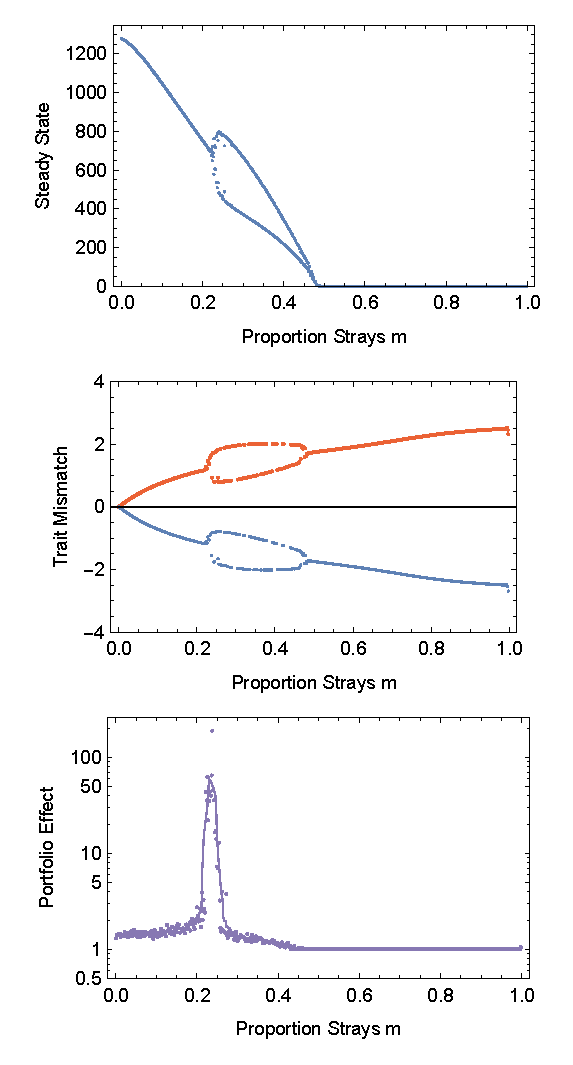
\includegraphics[width=0.4\textwidth]{figs/fig_Density.pdf}
\caption{} \label{fig:traj}
\end{figure}


The differences in optimal trait values between sites ($\theta_i-\theta_j$) influence at what straying rate the alternative stable states appear.
Large differences in $\theta_i$ and $\theta_j$ can be interpreted as high environmental heterogeneity.
A cursory analysis shows that increasing environmental heterogeneity tends to lower the stray rate value $m^*$ at which the maximum PE is expected to occur.
Moreover, if the trait variance is much larger than the difference in optimal trait values between sites (such that selection is weaker), the alternative stable state phenomenon disappears, as does the spike in the portfolio effect.


\begin{figure}[h]
\centering
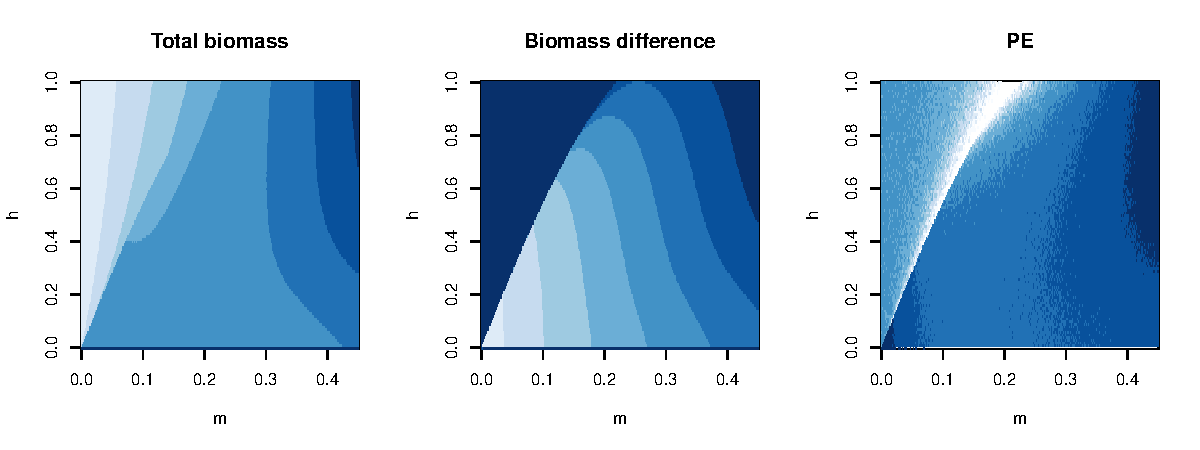
\includegraphics[width=0.8\textwidth]{figs/fig_MDPE_hm.pdf}
\caption{} \label{fig:PE}
\end{figure}



\begin{figure}
\centering
\begin{subfigure}[t]{0.8\textwidth}
\centering
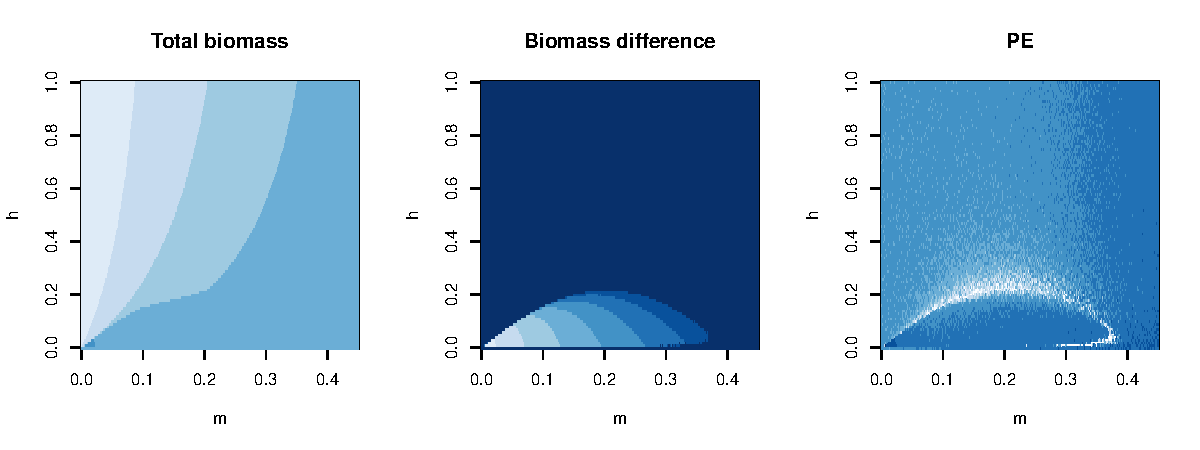
\includegraphics[width=\textwidth]{figs/fig_MDPE_hm_theta3.pdf} 
\caption{Low habitat heterogeneity ($\Delta\theta=3$)} \label{fig:hetero1}
\end{subfigure}

\begin{subfigure}[t]{0.8\textwidth}
\centering
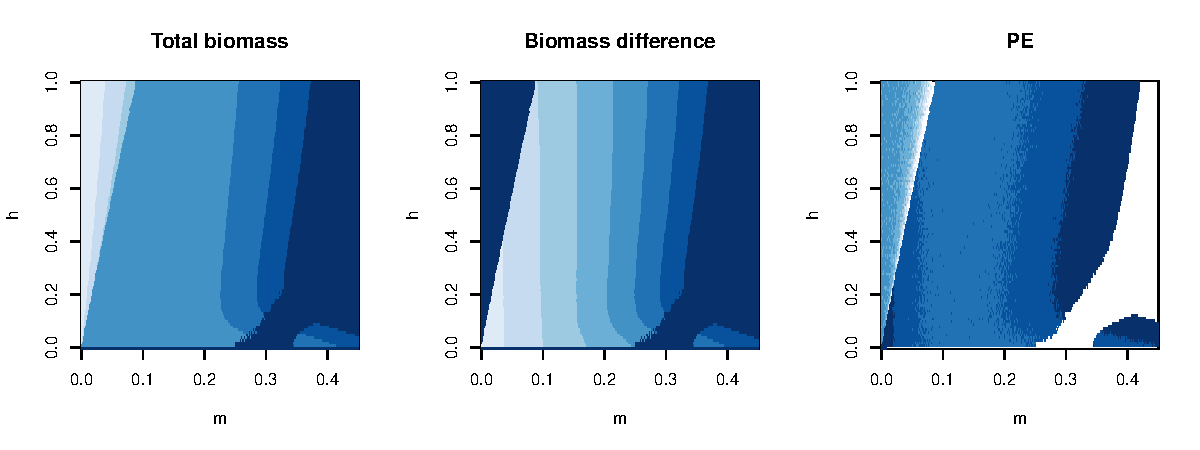
\includegraphics[width=\textwidth]{figs/fig_MDPE_hm_theta8.pdf} 
\caption{High habitat heterogeneity ($\Delta\theta=8$)} \label{fig:hetero2}
\end{subfigure}

 \caption{Changes in total means, difference in means, and the portfolio effect for different habitat heterogeneities}

\end{figure}

\begin{figure}[h]
\centering
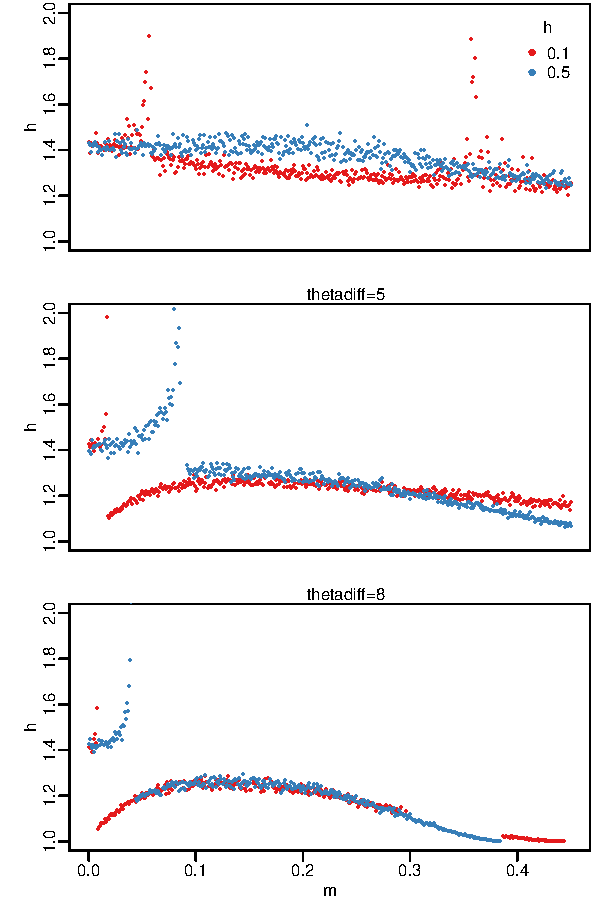
\includegraphics[width=0.5\textwidth]{figs/fig_MDPE_hm_cross358.pdf}
\caption{} \label{fig:PE}
\end{figure}


\section*{Discussion}

\end{document}
